%----------------------------------------------------------------------------
%
%	This template was created by
%		Christian Krieg <christian.krieg@alumni.tuwien.ac.at>
%
%	April 2018
%
%----------------------------------------------------------------------------
%
\documentclass[%
	a4paper,
]
{article}
%
%----------------------------------------------------------------------------
%
% Institution
%
%\institution{Institute of Computer Technology}
%
%----------------------------------------------------------------------------
%
% Use the 'Libertine' font type
%
\usepackage{libertine}
\usepackage[T1]{fontenc}
\usepackage[utf8]{inputenc}
%
%----------------------------------------------------------------------------
%
% Set page margins
%
\usepackage{geometry}
\geometry{%
	left   = 2cm,
	right  = 2cm,
	top    = 2cm,
	bottom = 2cm
}
%
%----------------------------------------------------------------------------
%
% Set line spacing
%
\usepackage{setspace}
\setstretch{1}
%
%----------------------------------------------------------------------------
%
% Settings for hyperlinks
%
\usepackage{hyperref}
\hypersetup{%
	colorlinks = true,
	allcolors  = blue,
}
%
%----------------------------------------------------------------------------
%
% Use colors
%
\usepackage{xcolor}
\usepackage{colortbl}
%
%----------------------------------------------------------------------------
%
% Define a TODO and a DONE command
%
\newcommand{\todo}[1]{\textcolor{red}{#1}}
\newcommand{\done}[1]{}
%
%----------------------------------------------------------------------------
%
% Use glossaries
%
\usepackage{glossaries}
\makeglossaries
%
% Glossary entries
%
\newglossaryentry{fpga}{
	name = {FPGA},
	description = {Field-programmable gate array},
	text = {FPGA},
	first = {field-programmable gate array (FPGA)},
	plural = {FPGAs},
	firstplural = {field-programmable gate arrays (FPGAs)},
}
%
\newglossaryentry{trng}{
	name = {TRNG},
	description = {True-random number generator},
	text = {TRNG},
	first = {true-random number generator (TRNG)},
	plural = {TRNGs},
	firstplural = {true-random number generators (TRNGs)},
}
%
\newglossaryentry{bcd}{
  name={BCD},
  description={Binary-coded decimal},
  text={BCD},
  first={binary-coded decimal (BCD)},
}
%
\newglossaryentry{hdl}{
  name={HDL},
  description={Hardware description language},
  text={HDL},
  first={hardware description language (HDL)},
  plural={HDLs},
  firstplural={hardware description languages (HDLs)},
}
%
\newglossaryentry{ip}{
  name={IP},
  description={Intellectual property},
  text={IP},
  first={intellectual property (IP)},
}
%
\newglossaryentry{3pip}{
  name={3PIP},
  description={Third-party intellectual property},
  text={3PIP},
  first={third-party intellectual property (3PIP)},
}
%
\newglossaryentry{dsp}{
  name={DSP},
  description={Digital signal processor},
  text={DSP},
  first={digital signal processor (DSP)},
  plural={DSPs},
  firstplural={digital signal processors (DSPs)},
}
%
\newglossaryentry{led}{
  name={LED},
  description={Light emitting diode},
  text={LED},
  first={light emitting diode (LED)},
  plural={LEDs},
  firstplural={light emitting diodes (LEDs)},
}
%
%\newglossaryentry{}{
%  name={},
%  description={},
%  text={},
%  first={},
%  plural={},
%  firstplural={},
%}
%
%----------------------------------------------------------------------------
%
% Settings for citations and the bibliography
%
\usepackage[%
	backend     = biber,
	maxbibnames = 99,
	autocite    = footnote,
	citestyle   = verbose-ibid,
	firstinits=true,
]{biblatex}
\bibliography{bib/report}
%
%----------------------------------------------------------------------------
%
%	TikZ -- TikZ ist kein Zeichenprogramm
%
\usepackage{tikz}
\usepackage{tikz-timing}
\usepackage{etoolbox}
\usetikzlibrary{mindmap}
\usetikzlibrary{shapes}
\usetikzlibrary{arrows}
\usetikzlibrary{decorations}
\usetikzlibrary{shapes.symbols}
\usetikzlibrary{shapes.geometric}
\usetikzlibrary{shapes.multipart}
\usetikzlibrary{positioning}
\usetikzlibrary{patterns}
\usetikzlibrary{calc}
\usetikzlibrary{scopes}         % cf. pgfmanual p.66
\usetikzlibrary{chains}         % cf. pgfmanual p.284
\usetikzlibrary{fit}
\usetikzlibrary{matrix}
\usetikzlibrary{decorations}
\usetikzlibrary{circuits.logic}
\usetikzlibrary{circuits.logic.IEC}
\usetikzlibrary{shapes.gates.logic.IEC}
\usetikzlibrary{circuits.logic.US}
\usetikzlibrary{shapes.gates.logic.US}
\usetikzlibrary{circuits.ee}
\usetikzlibrary{circuits.ee.IEC}
\usetikzlibrary{backgrounds}
\usetikzlibrary{automata}
\usetikzlibrary{intersections}
\usetikzlibrary{plotmarks}
\usepgflibrary{fpu}
\usetikzlibrary{decorations.pathreplacing}
%
%----------------------------------------------------------------------------
%
% TikZ shapes
%  
	% D flip-flops (DFFs) and shift register
% Author: Martin Scharrer
%\documentclass[a4paper,landscape]{article}

%\usepackage{pgf,tikz}
%%%<
%\usepackage{verbatim}
%\usepackage[active,tightpage]{preview}
%\PreviewEnvironment{tikzpicture}
%\setlength\PreviewBorder{5pt}%
%%%>

%\begin{comment}
%:Title: D flip-flops and shift register
%
%Example of a custom node shape for drawing  D flip-flops. The shape is used to draw a serial shift
%register. 
%
%\end{comment}
%
%\usetikzlibrary{calc,arrows}
%\usepackage{amsmath}
%\usepackage[left=1cm,right=1cm]{geometry}
%\pagestyle{empty}

\makeatletter

% Data Flip Flip (DFF) shape
\pgfdeclareshape{dff}{
  % The 'minimum width' and 'minimum height' keys, not the content, determine
  % the size
  \savedanchor\northeast{%
    \pgfmathsetlength\pgf@x{\pgfshapeminwidth}%
    \pgfmathsetlength\pgf@y{\pgfshapeminheight}%
    \pgf@x=0.5\pgf@x
    \pgf@y=0.5\pgf@y
  }
  % This is redundant, but makes some things easier:
  \savedanchor\southwest{%
    \pgfmathsetlength\pgf@x{\pgfshapeminwidth}%
    \pgfmathsetlength\pgf@y{\pgfshapeminheight}%
    \pgf@x=-0.5\pgf@x
    \pgf@y=-0.5\pgf@y
  }
  % Inherit from rectangle
  \inheritanchorborder[from=rectangle]

  % Define same anchor a normal rectangle has
  \anchor{center}{\pgfpointorigin}
  \anchor{north}{\northeast \pgf@x=0pt}
  \anchor{east}{\northeast \pgf@y=0pt}
  \anchor{south}{\southwest \pgf@x=0pt}
  \anchor{west}{\southwest \pgf@y=0pt}
  \anchor{north east}{\northeast}
  \anchor{north west}{\northeast \pgf@x=-\pgf@x}
  \anchor{south west}{\southwest}
  \anchor{south east}{\southwest \pgf@x=-\pgf@x}
  \anchor{text}{
    \pgfpointorigin
    \advance\pgf@x by -.5\wd\pgfnodeparttextbox%
    \advance\pgf@y by -.5\ht\pgfnodeparttextbox%
    \advance\pgf@y by +.5\dp\pgfnodeparttextbox%
  }

  % Define anchors for signal ports
  \anchor{D}{
    \pgf@process{\northeast}%
    \pgf@x=-1\pgf@x%
    \pgf@y=.5\pgf@y%
  }
  \anchor{CLK}{
    \pgf@process{\northeast}%
    \pgf@x=-1\pgf@x%
    \pgf@y=-.66666\pgf@y%
  }
  \anchor{CE}{
    \pgf@process{\northeast}%
    \pgf@x=-1\pgf@x%
    \pgf@y=-0.33333\pgf@y%
  }
  \anchor{Q}{
    \pgf@process{\northeast}%
    \pgf@y=.5\pgf@y%
  }
  \anchor{Qn}{
    \pgf@process{\northeast}%
    \pgf@y=-.5\pgf@y%
  }
  \anchor{R}{
    \pgf@process{\northeast}%
    \pgf@x=0pt%
  }
  \anchor{S}{
    \pgf@process{\northeast}%
    \pgf@x=0pt%
    \pgf@y=-\pgf@y%
  }
  % Draw the rectangle box and the port labels
  \backgroundpath{
    % Rectangle box
    \pgfpathrectanglecorners{\southwest}{\northeast}
    % Angle (>) for clock input
    \pgf@anchor@dff@CLK
    \pgf@xa=\pgf@x \pgf@ya=\pgf@y
    \pgf@xb=\pgf@x \pgf@yb=\pgf@y
    \pgf@xc=\pgf@x \pgf@yc=\pgf@y
    \pgfmathsetlength\pgf@x{.75ex} % size depends on font size
    \advance\pgf@ya by \pgf@x
    \advance\pgf@xb by \pgf@x
    \advance\pgf@yc by -\pgf@x
    \pgfpathmoveto{\pgfpoint{\pgf@xa}{\pgf@ya}}
    \pgfpathlineto{\pgfpoint{\pgf@xb}{\pgf@yb}}
    \pgfpathlineto{\pgfpoint{\pgf@xc}{\pgf@yc}}
    \pgfclosepath

    % Draw port labels
    \begingroup
    \tikzset{flip flop/port labels} % Use font from this style
    \tikz@textfont

    \pgf@anchor@dff@D
    \pgftext[left,base,at={\pgfpoint{\pgf@x}{\pgf@y}},x=\pgfshapeinnerxsep]{\raisebox{-0.75ex}{D}}

%    \pgf@anchor@dff@CE
%    \pgftext[left,base,at={\pgfpoint{\pgf@x}{\pgf@y}},x=\pgfshapeinnerxsep]{\raisebox{-0.75ex}{CE}}

    \pgf@anchor@dff@Q
    \pgftext[right,base,at={\pgfpoint{\pgf@x}{\pgf@y}},x=-\pgfshapeinnerxsep]{\raisebox{-.75ex}{Q}}

%    \pgf@anchor@dff@Qn
%    \pgftext[right,base,at={\pgfpoint{\pgf@x}{\pgf@y}},x=-\pgfshapeinnerxsep]{\raisebox{-.75ex}{$\overline{\mbox{Q}}$}}
%
%    \pgf@anchor@dff@R
%    \pgftext[top,at={\pgfpoint{\pgf@x}{\pgf@y}},y=-\pgfshapeinnerysep]{R}
%
%    \pgf@anchor@dff@S
%    \pgftext[bottom,at={\pgfpoint{\pgf@x}{\pgf@y}},y=\pgfshapeinnerysep]{S}
    \endgroup
  }
}

% Key to add font macros to the current font
\tikzset{add font/.code={\expandafter\def\expandafter\tikz@textfont\expandafter{\tikz@textfont#1}}} 

% Define default style for this node
% \tikzset{flip flop/port labels/.style={font=\sffamily\scriptsize}}
%\tikzset{every dff node/.style={draw,minimum width=2cm,minimum 
%height=2.828427125cm,very thick,inner sep=1mm,outer sep=0pt,cap=round,add 
%font=\sffamily}}
\tikzset{flip flop/port labels/.style={font=\tiny}}
\tikzset{every dff node/.style={draw,minimum width=.75cm,minimum 
height=1cm,inner sep=1mm,outer sep=0pt,cap=round,font=\scriptsize}}

\makeatother

%\begin{document}
%
%\begin{tikzpicture}[font=\sffamily,>=triangle 45]
%  \def\N{7}  % Number of Flip-Flops minus one
%
%  % Place FFs
%  \foreach \m in {0,...,\N}
%    \node [shape=dff] (DFF\m) at ($ 3*(\m,0) $) {Bit \#\m};
%
%  % Connect FFs (Q1 with D1, etc.)
%  \def\p{0}  % Used to save the previous number
%  \foreach \m in {1,...,\N} { % Note that it starts with 1, not 0
%    \draw [->] (DFF\p.Q) -- (DFF\m.D);
%    \global\let\p\m
%  }
%
%  % Connect and label data in- and output port
%  \draw [<-] (DFF0.D) -- +(-1,0) node [anchor=east] {input} ;
%  \draw [->] (DFF\N.Q) -- +(1,0) node [anchor=west] {output};
%
%  % 'Reset' port label
%  \path (DFF0) +(-2cm,+2cm) coordinate (temp)
%    node [anchor=east] {reset};
%  % Connect resets
%  \foreach \m in {0,...,\N}
%    \draw [->] (temp) -| (DFF\m.R);
%
%  % 'Set' port label
%  \path (DFF0) +(-2cm,-2cm) coordinate (temp)
%    node [anchor=east] {set};
%  % Connect sets
%  \foreach \m in {0,...,\N}
%    \draw [->] (temp) -| (DFF\m.S);
%
%  % Clock port label
%  \path (DFF0) +(-2cm,-2.5cm) coordinate (temp)
%    node [anchor=east] {clock};
%  \foreach \m in {0,...,\N}
%    \draw [->] (temp) -| ($ (DFF\m.CLK) + (-5mm,0) $) --(DFF\m.CLK);
%
%  % Clock port label
%  \path (DFF0) +(-2cm,-3cm) coordinate (temp)
%    node [anchor=east] {clock enable};
%  \foreach \m in {0,...,\N}
%    \draw [->] (temp) -| ($ (DFF\m.CE) + (-7.5mm,0) $) --(DFF\m.CE);
%\end{tikzpicture}
%
%\end{document}

%
%----------------------------------------------------------------------------
%
% Use AMS math fonts
%
\usepackage{amsfonts}
\usepackage[sans]{dsfont}
%
%----------------------------------------------------------------------------
%
% Use multiple figures in one float
%
\usepackage{subcaption}
%
%----------------------------------------------------------------------------
%
% Use dummy text
%
\usepackage{lipsum}
%
%----------------------------------------------------------------------------
%
% Use extended list environments (e.g., 'inparaenum')
%
\usepackage{paralist}
%
%----------------------------------------------------------------------------
%
% Use listings
%
\usepackage{listings}

\lstdefinestyle{vhdl}
{
	language=VHDL,
  basicstyle=\linespread{1}\scriptsize\ttfamily\color{black},
  commentstyle=\scriptsize\itshape,
  escapeinside={(*@}{@*)},
  frame=single, numbers=left,
%  numbersep=5pt,
  xleftmargin=15pt,
  xrightmargin=5pt,
  numbersep=5pt,
  breaklines=true,
  moredelim=**[is][\ttfamily\bfseries\color{red}]{(*}{*)},
}

\lstdefinestyle{verilog}
{
	language=Verilog,
  basicstyle=\linespread{1}\scriptsize\ttfamily\color{black},
  commentstyle=\scriptsize\itshape,
  escapeinside={(*@}{@*)},
  frame=single, numbers=left,
%  numbersep=5pt,
  xleftmargin=15pt,
  xrightmargin=5pt,
  numbersep=5pt,
  breaklines=true,
  moredelim=**[is][\ttfamily\bfseries\color{red}]{(*}{*)},
}
%
%----------------------------------------------------------------------------
%
% Typeset pseudo code
%
\usepackage{syntax}
%
%----------------------------------------------------------------------------
%
% More options for boxes
%
\usepackage{realboxes}
%
% Command for vertical text in tabulars
%
\newcommand*\rot{\rotatebox{90}}
%
%----------------------------------------------------------------------------
%
% Use \textsubscript
%
\usepackage{fixltx2e}
%
%----------------------------------------------------------------------------
%
% More options for tabulars
%
\usepackage{array}
%
%----------------------------------------------------------------------------
%
% Use appendices
%
\usepackage[titletoc]{appendix}
%
%----------------------------------------------------------------------------
%
% Use the cleverref package -- Load this package as the very last!
%
\usepackage{cleveref}
%
%----------------------------------------------------------------------------
%
% Document body
%
\begin{document}
%
%----------------------------------------------------------------------------
%
\begin{titlepage}

	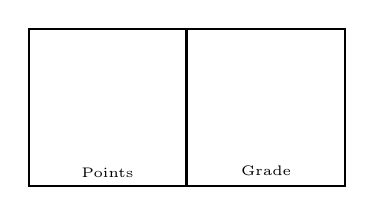
\begin{tikzpicture}[thick]
		\node (points) at (0,0) [draw,minimum size=2cm] {};
		\node (lbl-points) at (points.south) [anchor=south,font=\tiny] {Points};
		\node (grade) at (points.east) [draw,minimum size=2cm,anchor=west,
			outer sep=0] {};
		\node (lbl-grade) at (grade.south) [anchor=south,font=\tiny] {Grade};
	\end{tikzpicture}

	\begin{flushright}

		% Update this with your team number
		\huge\bfseries
		Team: XX \\[1em]

		% Update this with your matriculation number, first name, second name
		\large
		MatNr. First SECOND \#1	\\
		MatNr. First SECOND \#2	\\
		... \\
	
	\end{flushright}

	\vspace{5em}

	\begin{center}
		{\huge Digital Integrated Circuits Lab (LDIS)}\\[1em]
		{\Large 384.088, Summer Term 2019} \\[2em]
		{\large Supervisors:\\[.5em]
			Christian Krieg, David Radakovits, Axel Jantsch} \\[10em]

		{\Huge Task 1: Digital Waterscale}\\[10em]
	\end{center}


%	\begin{abstract}
%
%		Enter the abstract of your report here. An abstract summarizes your
%		entire work (i.e., problem statement, motivation, methodology, key
%		findings). It is a good strategy to write a first version of the abstract
%		when you start to work on your report. This gives you a good guideline
%		what to	put and what not to put into the report. Ideally, you re-write
%		the abstract once you finished your report, because only at this point
%		you have all the information available to create a good abstract.
%
%	\end{abstract}

\end{titlepage}
%
%----------------------------------------------------------------------------
%
\section{Problem statement}

Your goal is to design a system that reads data from an accelerometer,
performs simple digital signal processing on captured data, and outputs the
processed signal via \gls{led} bar (\Cref{fig:block}).

\begin{figure}[h!]
	\centering
	\input{fig/block}
	\caption{Block diagram of the system}
	\label{fig:block}
\end{figure}

\noindent
You have to design three \gls{ip} cores:

\begin{enumerate}

	\item{Data sampling: This \gls{ip} core controls and reads the output of
		the accelerometer, and provides the sampled data of a pre-defined sample
		rate at its output. The sample rate should be adjustable pre-synthesis.
		The	accelerometer signal's resolution should be 12-bit.}

	\item{The \gls{dsp} core should implement an algorithm that calculates
		the angle of the board relative to the horizon in the axis of the
		\gls{led} bar.}

	\item{The output stage takes the calculated angle, and transforms it into
		a thermometer-encoded signal that is provided to the \gls{led} bar.
		If the \gls{led} bar is parallel to the horizon, all \glspl{led}
		should be turned off. If the led bar is tilted perpendicular both to the
		horizon and the ground, the entire upper portion of the \gls{led} bar
		should be turned on. If the angle of the board is between 0 and 90
		degrees, the corresponding share of the \glspl{led} should
		be turned on.}

\end{enumerate}

\noindent
Design the system using either VHDL or Verilog. You can use \gls{3pip}, but
you have to fully understand what you are doing, and you have to cite the
original source.
%
%----------------------------------------------------------------------------
%
\section{Team management}

You can solve the problem on your own, or you can team up with others in
order to share work and knowledge. If you team up, it is essential that you
understand every aspect of the solution, rather that just the part that was
implemented by you.
%
In any case, use \emph{git} to organize collaboration, even in case you work
alone. We will assess your activity in the project based on your commits.
%
%----------------------------------------------------------------------------
%
\section{Proposed solution}

Model the system in any \gls{hdl} of your choice. Design a testbench with
reasonable test cases, and verify the design's functional correctness by
simulating
your design. Use any simulator you prefer, however, support is only provided
for \emph{ghdl}, \emph{Verilator}, \emph{Icarus Verilog}, and
\emph{xsim}. You can use free and open-source tools for modeling, simulation
and synthesis. However, for technology mapping and bitstream generation (i.e.,
\emph{implementing} the design), you will need \emph{Vivado}.
Implement the design on the Nexys 4 DDR board.

%
%----------------------------------------------------------------------------
%
\end{document}
%
%----------------------------------------------------------------------------
